\chapter{Validation of the Replicated Analytical Configurations}
\label{chap:validation_results}

\section{Chapter Overview}

This chapter evaluates the final analytical configurations established after completion of the replication stage. The heart disease, stroke, diabetes, and \gls{ckd} experiments use held-out test partitions. The \gls{hbaone} experiment retains the full-cohort inferential design of its source study and is therefore excluded from comparisons of held-out predictive performance \citep{strack_impact_2014}. The four predictive experiments reuse the test partitions established in their dataset-specific workflows. Their results constitute internal held-out evaluation rather than external or prospective clinical validation \citep{collins_tripodai_2024, moons_probastai_2025}.

The final model configurations were specified without using their held-out test rankings as a retrospective selection criterion. This separation reduces the risk of adapting model choices to test-set performance \citep{collins_tripodai_2024, moons_probastai_2025}. To ensure consistency across analyses, the uncertainty analysis loaded the fitted models and aligned test data exported by the \gls{xai}-extension notebooks. This technical execution sequence does not alter the analytical logic of the dissertation. Predictive performance and its uncertainty are evaluated before the corresponding explanation results are interpreted.


\section{\gls{ckd} Preprocessing Comparison}

The paper-style \gls{ckd} replication fitted missing-value imputation and categorical encoding using the complete dataset before creating the training and test partitions, following the reconstructed source workflow \citep{santhiya_chronic_2024}. In the leakage-controlled workflow, the data were partitioned first. The imputation parameters and categorical encoding structure were then learned exclusively from the training observations and applied to the test observations. This separation prevents test-set information from contributing to model development \citep{collins_tripodai_2024, moons_probastai_2025}.

Applying both preprocessing orders to the same stratified partition produced the model-specific accuracy differences shown in Table~\ref{tab:ckd_leakage_comparison}.

\begin{table}[htbp]
    \centering
    \small
    \caption{\gls{ckd} test accuracy under leakage-controlled and paper-style preprocessing. Difference denotes paper-style accuracy minus leakage-controlled accuracy, with both workflows evaluated using the same train--test partition.}
    \label{tab:ckd_leakage_comparison}
    \begin{tabular}{@{}lrrr@{}}
        \toprule
        \textbf{Model} & \textbf{Leakage-controlled} & \textbf{Paper-style} & \textbf{Difference$^{a}$} \\
        \midrule
        \Gls{rf} & 0.983 & 0.992 & +0.009 \\
        Gradient boosting & 0.967 & 0.992 & +0.025 \\
        Gaussian naive Bayes & 0.958 & 0.942 & -0.016 \\
        \Gls{dt} & 0.942 & 0.983 & +0.041 \\
        \Gls{knn} & 0.658 & 0.650 & -0.008 \\
        \bottomrule
        \multicolumn{4}{@{}l@{}}{\footnotesize
        $^{a}$ Paper-style accuracy minus leakage-controlled accuracy.}
    \end{tabular}
\end{table}

As shown in Table~\ref{tab:ckd_leakage_comparison}, the direction and magnitude of the difference varied across models. Paper-style preprocessing produced higher accuracy for \gls{rf}, gradient boosting, and \gls{dt}, while leakage-controlled preprocessing produced higher accuracy for Gaussian naive Bayes and \Gls{knn}. The methodological concern does not depend on whether the observed score increases or decreases. When the complete dataset determines preprocessing parameters, information from the test observations contributes to the fitted analytical pipeline, and the test partition is no longer fully independent \citep{collins_tripodai_2024, moons_probastai_2025}. The leakage-controlled \gls{rf} was therefore used for the held-out predictive evaluation and subsequent \gls{xai} extension.

The unusually high \gls{ckd} scores were also checked for exact record duplication. The 400 rows had unique identifiers; no predictor--outcome row was duplicated after removal of the identifier; and no identical predictor profile occurred in both the stratified training and test partitions. The same checks after training-fitted imputation and encoding found no exact duplicates within either partition and no exact cross-partition profile overlap. Exact duplication therefore did not explain the near-perfect internal results, although the small dataset remains unusually separable and requires external validation.

\section{Held-Out Analytical Configurations}

The four final predictive configurations were evaluated on the held-out test partitions established in their dataset-specific workflows. Model choice was specified independently of the observed test rankings to preserve the test data for evaluation \citep{collins_tripodai_2024, moons_probastai_2025}. Table~\ref{tab:final_model_metrics} brings together the resulting point estimates and allows the performance profiles of the four configurations to be compared. \gls{hbaone} is presented separately because its source study fitted an inferential logistic-regression model to the complete eligible cohort rather than evaluating predictive performance on held-out observations \citep{strack_impact_2014}.

\begin{table}[htbp]
    \centering
    \small
    \caption{Final predictive configurations and point estimates for the four models evaluated on held-out test data. \gls{hbaone} is excluded because its full-cohort inferential design did not provide an independent test partition.}
    \label{tab:final_model_metrics}
    \setlength{\tabcolsep}{4pt}
    \begin{tabular}{@{}llrrrrrr@{}}
        \toprule
        \textbf{Dataset} &
        \textbf{Final model} &
        \textbf{$n_{\mathrm{test}}$} &
        \textbf{Accuracy} &
        \textbf{Precision} &
        \textbf{Recall} &
        \textbf{F1} &
        \textbf{\gls{rocauc}} \\
        \midrule
        Heart &
        Logistic regression (10-fold \gls{cv}) &
        149 & 0.852 & 0.841 & 0.841 & 0.841 & 0.915 \\
        Stroke &
        Balanced logistic regression &
        1,022 & 0.754 & 0.142 & 0.800 & 0.242 & 0.834 \\
        Diabetes &
        \Gls{rf}, five features &
        230 & 0.752 & 0.658 & 0.600 & 0.627 & 0.816 \\
        \gls{ckd} &
        \Gls{rf} &
        120 & 0.983 & 0.987 & 0.987 & 0.987 & 0.999 \\
        \bottomrule
    \end{tabular}
\end{table}

As shown in Table~\ref{tab:final_model_metrics}, the four configurations exhibited different performance profiles. The heart-disease model combined high discrimination with similar precision, recall, and F1 scores. The balanced stroke model prioritised sensitivity, achieving a recall of 0.800 at the cost of low precision. The diabetes model produced moderate discrimination and classification performance. The \gls{ckd} model achieved near-perfect point estimates, although these estimates were based on the smallest held-out test partition, containing 120 observations. These differences demonstrate why evaluation should consider several complementary metrics rather than rely on a single measure \citep{powers_evaluation_2011, saito_precision-recall_2015}.

\section{Predictive Performance and Bootstrap Uncertainty}\label{sec:bootstrap_uncertainty}

Figure~\ref{fig:predictive_performance} compares accuracy, F1, \gls{rocauc}, and \gls{ap} across the four held-out configurations. \gls{ap} was calculated using the average-precision estimator rather than trapezoidal integration of the precision-recall curve. This distinction is relevant because precision-recall summaries are particularly informative when the positive outcome is uncommon \citep{saito_precision-recall_2015}. The corresponding \gls{ap} values were 0.912 for Heart, 0.220 for Stroke, 0.689 for Diabetes, and 0.999 for \gls{ckd}.

Uncertainty was estimated using a non-parametric observation-level percentile bootstrap with 5,000 resamples and random seed 42 \citep{efron_introduction_1993}. Within each test partition, observed labels and their corresponding predicted probabilities were resampled together while the fitted model remained fixed. The 2.5th and 97.5th percentiles formed the 95\% \gls{ci}. All 5,000 resamples produced valid metric values for each dataset. These intervals quantify variation associated with the observed test samples, conditional on the fixed fitted models. They do not incorporate uncertainty arising from model selection, model retraining, or changes in the target population.


\begin{figure}[H]
    \centering
    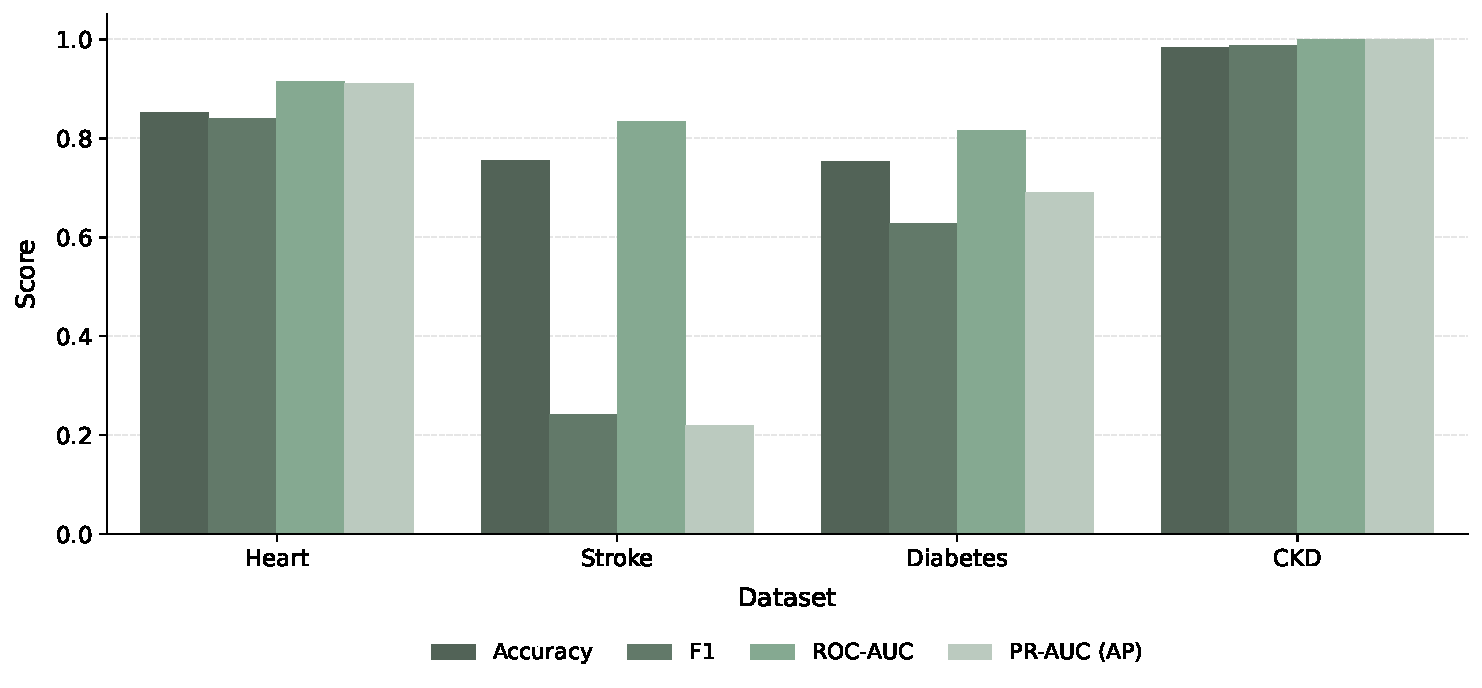
\includegraphics[width=1\textwidth]
    {images/results/predictive_performance.pdf}
    \caption{Held-out predictive performance of the four final models. Values should be interpreted within each dataset. Differences between datasets cannot be attributed solely to model family because the tasks, outcome prevalences, and evaluation samples differ.}
    \label{fig:predictive_performance}
\end{figure}

The numerical point estimates and bootstrap intervals are presented in Table~\ref{tab:bootstrap_performance_new}. Figure~\ref{fig:bootstrap_roc_auc} complements the table by displaying \gls{rocauc} separately, making differences in interval width easier to examine.

\begin{table}[H]
    \centering
    \small
    \renewcommand{\arraystretch}{1}
    \setlength{\tabcolsep}{8pt}
    \caption{Held-out performance with 95\% percentile bootstrap confidence intervals based on 5,000 observation-level resamples.}
    \label{tab:bootstrap_performance_new}
    \begin{tabular}{@{}lcccc@{}}
        \toprule
        \textbf{Dataset}
        & \textbf{Accuracy}
        & \textbf{F1}
        & \textbf{\gls{rocauc}}
        & \textbf{\gls{ap}} \\
        \midrule
        Heart
        & \shortstack{0.852 {[0.792, 0.906]}}
        & \shortstack{0.841 {[0.767, 0.903]}}
        & \shortstack{0.915 {[0.865, 0.956]}}
        & \shortstack{0.912 {[0.849, 0.959]}} \\

        Stroke
        & \shortstack{0.754 {[0.728, 0.780]}}
        & \shortstack{0.242 {[0.181, 0.303]}}
        & \shortstack{0.834 {[0.774, 0.887]}}
        & \shortstack{0.220 {[0.147, 0.339]}} \\

        Diabetes
        & \shortstack{0.752 {[0.696, 0.804]}}
        & \shortstack{0.627 {[0.531, 0.710]}}
        & \shortstack{0.816 {[0.757, 0.867]}}
        & \shortstack{0.689 {[0.586, 0.790]}} \\

        \gls{ckd}
        & \shortstack{0.983 {[0.958, 1.000]}}
        & \shortstack{0.987 {[0.965, 1.000]}}
        & \shortstack{0.999 {[0.996, 1.000]}}
        & \shortstack{0.999 {[0.998, 1.000]}} \\
        \bottomrule
    \end{tabular}
\end{table}

\begin{figure}[H]
    \centering
    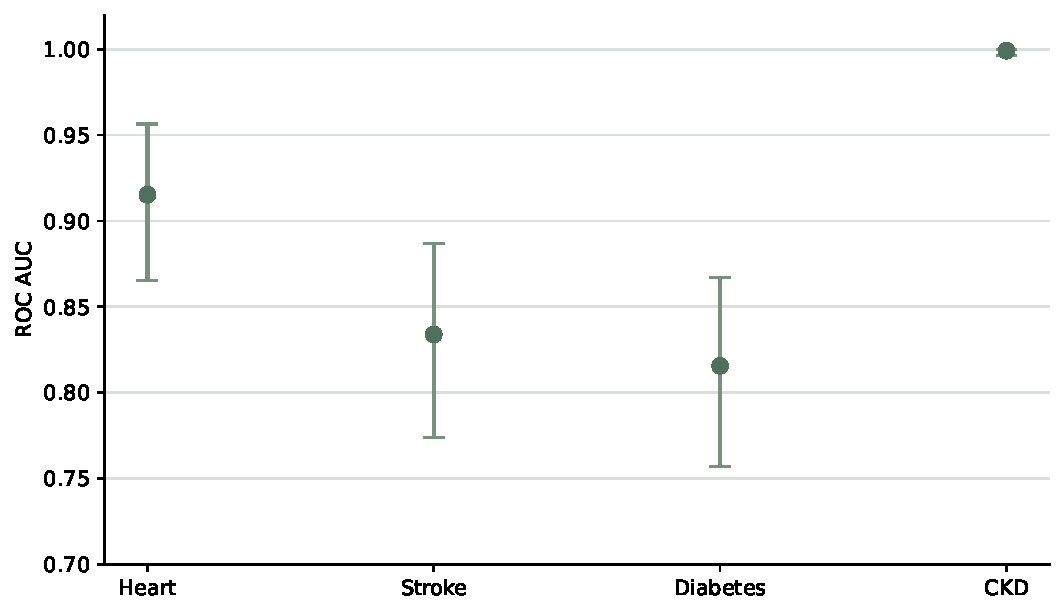
\includegraphics[width=\textwidth]{images/results/bootstrap_roc_auc.pdf}
    \caption{\gls{rocauc} point estimates and 95\% percentile bootstrap confidence intervals for the four models evaluated on held-out test data. The intervals represent uncertainty associated with the observed test samples while holding each fitted model fixed.}
    \label{fig:bootstrap_roc_auc}
\end{figure}

Heart combined strong discrimination, with a \gls{rocauc} of 0.915 and a 95\% \gls{ci} of 0.865-0.956, with balanced precision and recall of 0.841. Diabetes showed moderate discrimination, with a \gls{rocauc} of 0.816 and a 95\% \gls{ci} of 0.757-0.867. Its F1 score was 0.627, with a 95\% \gls{ci} of 0.531-0.710.

Stroke demonstrates why discrimination and threshold-dependent classification metrics must be considered separately \citep{fawcett_introduction_2006, powers_evaluation_2011}. Its \gls{rocauc} was 0.834, with a 95\% \gls{ci} of 0.774-0.887, but its precision was only 0.142, with a 95\% \gls{ci} of 0.103--0.184. Recall remained high at 0.800, with a 95\% \gls{ci} of 0.686-0.906. Its \gls{ap} of 0.220, with a 95\% \gls{ci} of 0.147-0.339, further reveals the limited positive-class precision associated with this imbalanced outcome \citep{saito_precision-recall_2015}.

\gls{ckd} achieved the highest observed point estimates, with an accuracy of 0.983, an F1 score of 0.987, and a \gls{rocauc} of 0.999. These estimates describe performance on the fixed internal test partition and do not establish performance in an external clinical population \citep{collins_tripodai_2024, moons_probastai_2025}. Chapter~\ref{chap:xai_results} shows that \gls{ckd} also had the highest mean complete-ranking stability under bootstrap refitting, although its top-three overlap was lower than that of Diabetes. Predictive uncertainty and explanation stability remain distinct because the former resamples held-out observations for a fixed model, whereas the latter changes the composition of the training sample and refits the model \citep{lofstrom_meta_2022, canha_functionally-grounded_2025}.

\section{Validation Findings}

The held-out analyses demonstrated that the four predictive configurations had different performance profiles. The stroke model achieved high recall at the cost of low precision and average precision, while the near-perfect \gls{ckd} estimates were obtained from a small internal test partition and do not establish external generalisability. These differences provide the predictive context required to interpret the explanation results in Chapter~\ref{chap:xai_results}.

Bootstrap predictive uncertainty and bootstrap-refit explanation stability address different sources of variation. The predictive-uncertainty analysis resamples held-out observations while keeping the fitted model fixed. The stability analysis instead resamples the final training matrix, refits the model, and examines changes in permutation-importance rankings on the unchanged test set. Neither result can be inferred from the other.
